\chapter{Research Findings}
For the purpose of benchmarking the performance of the algorithms, a total of five stocks from the basket of uncorrelated stocks were selected. These were MSFT, CDE, NAVB, HRG, and HL. 

\begin{center}
    \includegraphics[width=\textwidth]{stocks.png}
    \captionof{figure}{Basket of stocks}
    \label{fig:nonfloat}
\end{center}

\begin{center}
    \begin{tabular}{ | l | l | l | | l | l | l | p{5cm} |}
    \hline
     & MSFT & CDE & NAVB & HRG & HL \\ \hline
    Mean & 16.983 & 57.716 & 3.000 & 13.328 & 7.154 \\ \hline
    Median & 18.656 & 36.700 & 1.250 & 7.190 & 6.196 \\ \hline
    Maximum & 63.620 & 213.178 & 22.000 & 89.340 & 23.830 \\ \hline
    Minimum & 0.061 & 1.730 & 0.080 & 1.725 & 0.486 \\ \hline
    Variance & 204.707 & 2807.852 & 18.445 & 249.105 & 18.445 \\ \hline
    Standard Deviation & 14.308 & 52.989 & 4.29 & 15.783 & 4.295 \\ \hline
    Skewness & 0.716 & 0.918 & 2.213 & 2.708 & 0.651 \\ \hline
    Kurtosis & 0.250 & -0.550 & 4.193 & 6.865 & -0.081 \\ \hline
    \hline
    \end{tabular}
    \captionof{table}{Equities Descriptive Statistics}
    \label{table:nonfloat}
\end{center}

\section{Time Series Analysis}

\subsection{Random Walk}

\begin{center}
    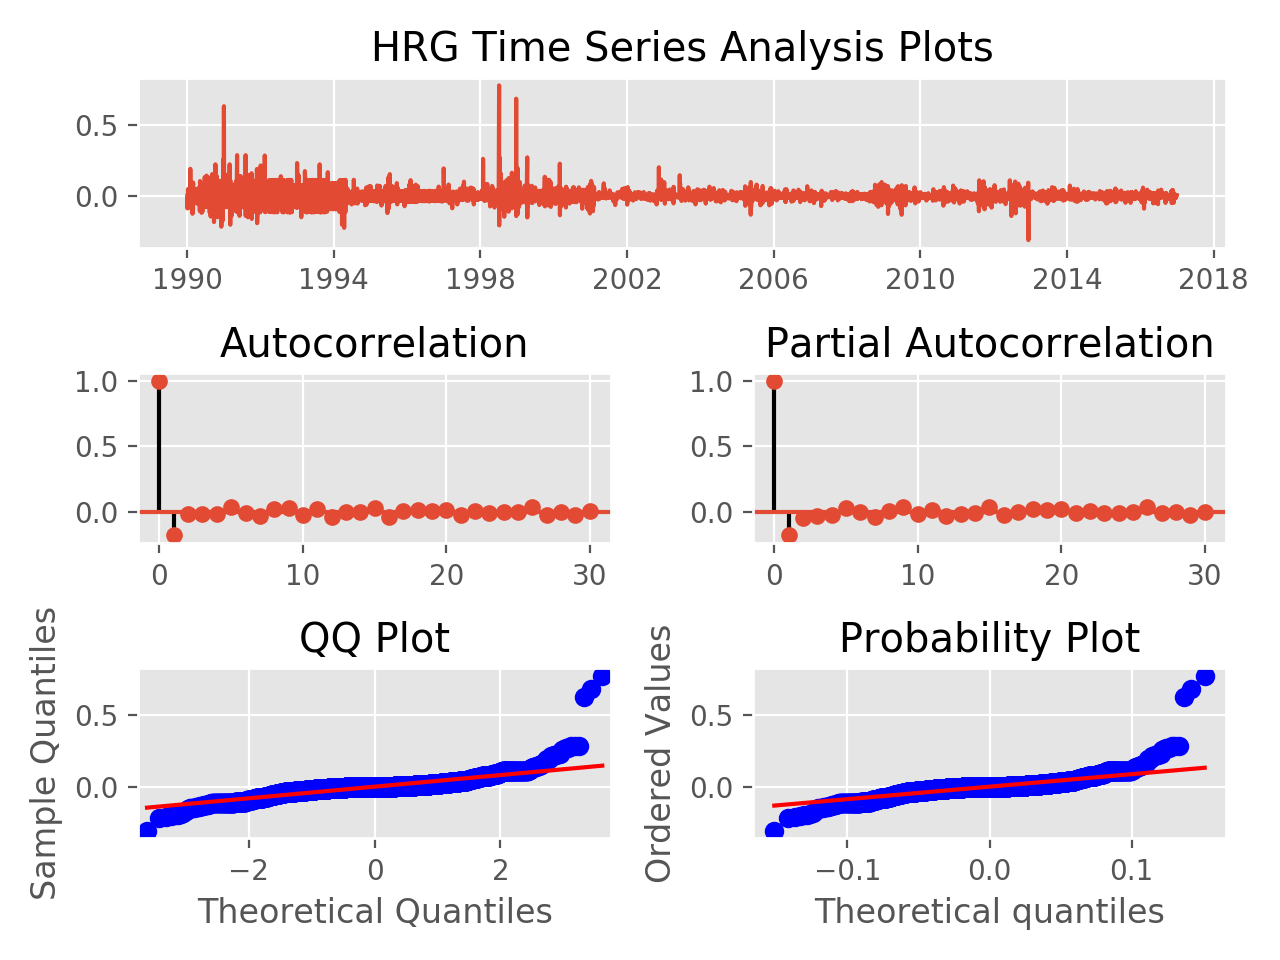
\includegraphics[width=\textwidth]{HRG-time-series.png}
    \captionof{figure}{HRG time series analysis}
    \label{fig:nonfloat}
\end{center}

\begin{center}  
    \includegraphics[width=\textwidth]{HRG-histogram.png}
    \captionof{figure}{HRG histogram of returns}
    \label{fig:nonfloat}
\end{center}

\subsection{Ordinary Least Squares (OLS)}
MSFT scored a mean absolute error regression loss of 0.810, and a coefficient of determination of 0.991.

\begin{center}
    \includegraphics[width=\textwidth]{MSFT-OLS-In-Sample-Prediction.png}
    \captionof{figure}{MSFT OLS in-sample prediction}
    \label{fig:nonfloat}
\end{center}

\begin{center}  
    \includegraphics[width=\textwidth]{100-Day-MSFT-OLS-Out-of-Sample-Forecast.png}
    \captionof{figure}{100 day MSFT OLS in-sample forecast}
    \label{fig:nonfloat}
\end{center}

\subsection{Auto Regressive (AR)}

MSFT scored sharpe ratios of 1.152 for the original returns, and -34.641 for the predicted returns in the in-sample test.

\begin{center}  
    \includegraphics[width=\textwidth]{MSFT-AR-time-series.png}
    \captionof{figure}{MSFT AR time series analysis}
    \label{fig:nonfloat}
\end{center}

\begin{center}
    \includegraphics[width=\textwidth]{MSFT-AR-histogram.png}
    \captionof{figure}{MSFT AR histogram of returns}
    \label{fig:nonfloat}
\end{center}

\begin{center}  
    \includegraphics[width=\textwidth]{MSFT-AR-In-Sample-Return-Prediction.png}
    \captionof{figure}{MSFT AR in-sample returns prediction}
    \label{fig:nonfloat}
\end{center}

\begin{center}
    \includegraphics[width=\textwidth]{100-Day-MSFT-AR-Out-of-Sample-Return-Forecast.png}
    \captionof{figure}{100 day MSFT AR in-sample returns forecast}
    \label{fig:nonfloat}
\end{center}

\subsection{Moving Average (MA)}

HRG scored sharpe ratios of 0.084 for the original returns, and -1.020 for the predicted returns in the in-sample test.

\begin{center}  
    \includegraphics[width=\textwidth]{HRG-MA-time-series.png}
    \captionof{figure}{HRG MA time series analysis}
    \label{fig:nonfloat}
\end{center}

\begin{center}  
    \includegraphics[width=\textwidth]{HRG-MA-histogram.png}
    \captionof{figure}{HRG MA histogram of returns}
    \label{fig:nonfloat}
\end{center}

\begin{center}
    \includegraphics[width=\textwidth]{HRG-MA-In-Sample-Return-Prediction.png}
    \captionof{figure}{HRG MA in-sample returns prediction}
    \label{fig:nonfloat}
\end{center}

\begin{center}
    \includegraphics[width=\textwidth]{100-Day-HRG-MA-Out-of-Sample-Return-Forecast.png}
    \captionof{figure}{100 day HRG MA in-sample returns forecast}
    \label{fig:nonfloat}
\end{center}

\subsection{Auto Regressive Moving Average (ARMA)}

CDE scored sharpe ratios of -0.128 for the original returns, and -0.977 for the predicted returns in the in-sample test.

\begin{center}
    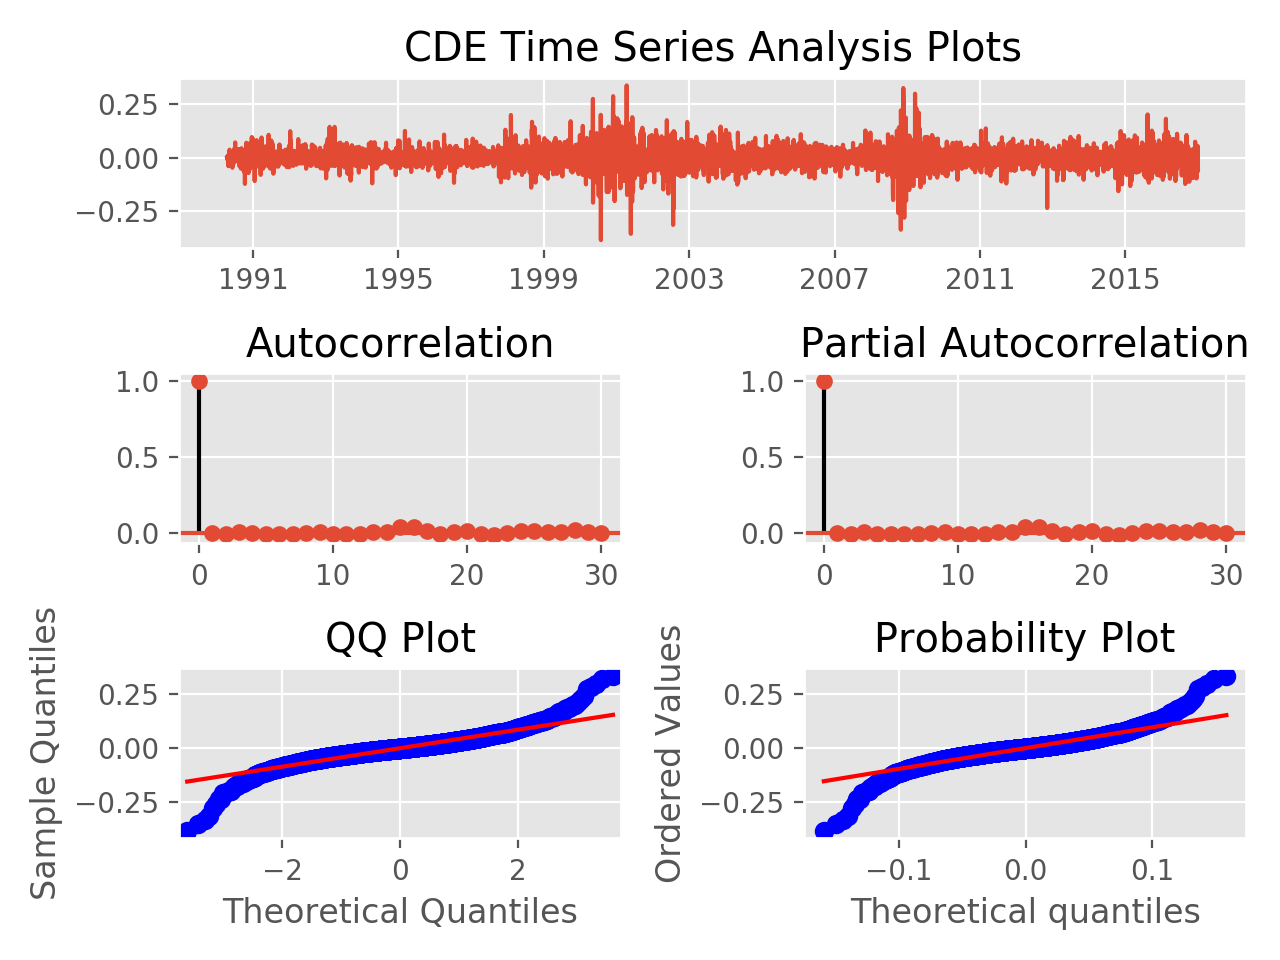
\includegraphics[width=\textwidth]{CDE-ARMA-time-series.png}
    \captionof{figure}{CDE ARMA time series analysis}
    \label{fig:nonfloat}
\end{center}

\begin{center}
    \includegraphics[width=\textwidth]{CDE-ARMA-histogram.png}
    \captionof{figure}{CDE ARMA histogram of returns}
    \label{fig:nonfloat}
\end{center}

\begin{center}
    \includegraphics[width=\textwidth]{CDE-ARMA-In-Sample-Return-Prediction.png}
    \captionof{figure}{CDE ARMA in-sample returns prediction}
    \label{fig:nonfloat}
\end{center}

\begin{center}
    \includegraphics[width=\textwidth]{100-Day-CDE-ARMA-Out-of-Sample-Return-Forecast.png}
    \captionof{figure}{100 day CDE ARMA in-sample returns forecast}
    \label{fig:nonfloat}
\end{center}

\subsection{Auto Regressive Integrated Moving Average (ARIMA)}

MSFT scored sharpe ratios of 0.123 for the original returns, and -4.904 for the predicted returns in the in-sample test.

\begin{center}  
    \includegraphics[width=\textwidth]{MSFT-ARIMA-time-series.png}
    \captionof{figure}{MSFT ARIMA time series analysis}
    \label{fig:nonfloat}
\end{center}

\begin{center}
    \includegraphics[width=\textwidth]{MSFT-ARIMA-histogram.png}
    \captionof{figure}{MSFT ARIMA histogram of returns}
    \label{fig:nonfloat}
\end{center}

\begin{center}  
    \includegraphics[width=\textwidth]{MSFT-ARIMA-In-Sample-Return-Prediction.png}
    \captionof{figure}{MSFT ARIMA in-sample returns prediction}
    \label{fig:nonfloat}
\end{center}

\begin{center}
    \includegraphics[width=\textwidth]{100-Day-MSFT-ARIMA-Out-of-Sample-Return-Forecast.png}
    \captionof{figure}{100 day MSFT ARIMA in-sample returns forecast}
    \label{fig:nonfloat}
\end{center}

\section{Machine Learning}

\subsection{Classification}

\subsubsection{Decision Tree}

\begin{center}
    \begin{tabular}{ | l | l | l | | l | l | l | p{5cm} |}
    \hline
    Ticker & Precision & True Negatives & False Negatives & True Positives & False Positives \\ \hline
    MSFT & 0.77 & 493 & 131 & 547 & 190 \\ \hline
    CDE & 0.79 & 565 & 144 & 504 & 133 \\ \hline
    NAVB & 0.76 & 592 & 165 & 331 & 126 \\ \hline
    HRG & 0.75 & 553 & 210 & 462 & 135 \\ \hline
    HL & 0.79 & 603 & 135 & 475 & 147 \\
    \hline
    \end{tabular}
    \captionof{table}{Decision Tree results}
    \label{table:nonfloat}
\end{center}

\subsubsection{Boosted Decision Tree}

\begin{center}
    \begin{tabular}{ | l | l | l | | l | l | l | p{5cm} |}
    \hline
    Ticker & Precision & True Negatives & False Negatives & True Positives & False Positives \\ \hline
    MSFT & 0.77 & 493 & 130 & 548 & 190 \\ \hline
    CDE & 0.79 & 564 & 143 & 505 & 134 \\ \hline
    NAVB & 0.76 & 588 & 164 & 332 & 130 \\ \hline
    HRG & 0.75 & 542 & 191 & 481 & 146 \\ \hline
    HL & 0.79 & 602 & 132 & 478 & 149 \\
    \hline
    \end{tabular}
    \captionof{table}{Boosted Decision Tree results}
    \label{table:nonfloat}
\end{center}

\subsubsection{Support Vector Machine (SVM)}

\begin{center}
    \begin{tabular}{ | l | l | l | | l | l | l | p{5cm} |}
    \hline
    Ticker & Precision & True Negatives & False Negatives & True Positives & False Positives \\ \hline
    MSFT & 0.77 & 493 & 130 & 548 & 190 \\ \hline
    CDE & 0.79 & 564 & 143 & 505 & 134 \\ \hline
    NAVB & 0.76 & 593 & 169 & 327 & 125 \\ \hline
    HRG & 0.75 & 542 & 191 & 481 & 146 \\ \hline
    HL & 0.81 & 579 & 98 & 512 & 171 \\
    \hline
    \end{tabular}
    \captionof{table}{Support Vector Machine results}
    \label{table:nonfloat}
\end{center}

\subsubsection{Random Forest}

\begin{center}    
    \begin{tabular}{ | l | l | l | | l | l | l | p{5cm} |}
    \hline
    Ticker & Precision & True Negatives & False Negatives & True Positives & False Positives \\ \hline
    MSFT & 0.77 & 493 & 131 & 547 & 190 \\ \hline
    CDE & 0.79 & 566 & 145 & 503 & 132 \\ \hline
    NAVB & 0.76 & 590 & 164 & 332 & 128 \\ \hline
    HRG & 0.75 & 554 & 210 & 462 & 134 \\ \hline
    HL & 0.81 & 581 & 101 & 509 & 169 \\
    \hline
    \end{tabular}
    \captionof{table}{Random Forest results}
    \label{table:nonfloat}
\end{center}

\subsubsection{K-Nearest Neighbour}

\begin{center}
    \begin{tabular}{ | l | l | l | | l | l | l | p{5cm} |}
    \hline
    Ticker & Precision & True Negatives & False Negatives & True Positives & False Positives \\ \hline
    MSFT & 0.76 & 489 & 130 & 548 & 194 \\ \hline
    CDE & 0.80 & 574 & 147 & 501 & 126 \\ \hline
    NAVB & 0.75 & 573 & 161 & 335 & 145 \\ \hline
    HRG & 0.74 & 560 & 233 & 439 & 128 \\ \hline
    HL & 0.81 & 581 & 101 & 509 & 169 \\
    \hline
    \end{tabular}
    \captionof{table}{K-Nearest Neighbour results}
    \label{table:nonfloat}
\end{center}

\subsubsection{Logistic Regression}

\begin{center}
    \begin{tabular}{ | l | l | l | | l | l | l | p{5cm} |}
    \hline
    Ticker & Precision & True Negatives & False Negatives & True Positives & False Positives \\ \hline
    MSFT & 0.77 & 493 & 130 & 548 & 190 \\ \hline
    CDE & 0.79 & 564 & 143 & 505 & 134 \\ \hline
    NAVB & 0.76 & 588 & 164 & 332 & 130 \\ \hline
    HRG & 0.75 & 542 & 191 & 481 & 146 \\ \hline
    HL & 0.79 & 601 & 132 & 478 & 149 \\
    \hline
    \end{tabular}
    \captionof{table}{Logistic Regression results}
    \label{table:nonfloat}
\end{center}

\subsubsection{Gaussian Naive Bayes}

\begin{center}
    \begin{tabular}{ | l | l | l | | l | l | l | p{5cm} |}
    \hline
    Ticker & Precision & True Negatives & False Negatives & True Positives & False Positives \\ \hline
    MSFT & 0.73 & 478 & 168 & 510 & 205 \\ \hline
    CDE & 0.76 & 555 & 187 & 461 & 143 \\ \hline
    NAVB & 0.74 & 553 & 153 & 343 & 165 \\ \hline
    HRG & 0.73 & 491 & 170 & 502 & 197 \\ \hline
    HL & 0.77 & 590 & 157 & 453 & 160 \\
    \hline
    \end{tabular}
    \captionof{table}{Gaussian Naive Bayes results}
    \label{table:nonfloat}
\end{center}

\subsubsection{Bernoulli Naive Bayes}

\begin{center}
    \begin{tabular}{ | l | l | l | | l | l | l | p{5cm} |}
    \hline
    Ticker & Precision & True Negatives & False Negatives & True Positives & False Positives \\ \hline
    MSFT & 0.73 & 479 & 169 & 509 & 204 \\ \hline
    CDE & 0.76 & 558 & 187 & 461 & 140 \\ \hline
    NAVB & 0.74 & 553 & 153 & 343 & 165 \\ \hline
    HRG & 0.73 & 492 & 170 & 502 & 196 \\ \hline
    HL & 0.77 & 590 & 158 & 452 & 160 \\
    \hline
    \end{tabular}
    \captionof{table}{Bernoulli Naive Bayes results}
    \label{table:nonfloat}
\end{center}

\subsubsection{Neural Network}

\begin{center}
    \begin{tabular}{ | l | l | l | | l | l | l | p{5cm} |}
    \hline
    Ticker & Precision & True Negatives & False Negatives & True Positives & False Positives \\ \hline
    MSFT & 0.77 & 685 & 181 & 787 & 258 \\ \hline
    CDE & 0.79 & 616 & 156 & 542 & 152 \\ \hline
    NAVB & 0.76 & 691 & 183 & 403 & 153 \\ \hline
    HRG & 0.74 & 690 & 269 & 542 & 164 \\ \hline
    HL & 0.77 & 1059 & 270 & 848 & 164 \\
    \hline
    \end{tabular}
    \captionof{table}{Neural Network results}
    \label{table:nonfloat}
\end{center}

\subsubsection{Stochastic Gradient Descent}

\begin{center}
    \begin{tabular}{ | l | l | l | | l | l | l | p{5cm} |}
    \hline
    Ticker & Precision & True Negatives & False Negatives & True Positives & False Positives \\ \hline
    MSFT & 0.77 & 493 & 130 & 548 & 190 \\ \hline
    CDE & 0.76 & 462 & 106 & 542 & 236 \\ \hline
    NAVB & 0.59 & 1032 & 707 & 118 & 80 \\ \hline
    HRG & 0.72 & 761 & 225 & 1059 & 518 \\ \hline
    HL & 0.80 & 535 & 83 & 527 & 215 \\
    \hline
    \end{tabular}
    \captionof{table}{Stochastic Gradient Descent results}
    \label{table:nonfloat}
\end{center}

\subsection{Regression}

\subsubsection{Decision Tree}
MSFT scored a mean absolute error regression loss of 5.606, and a coefficient of determination of 0.458.

\begin{center}
    \includegraphics[width=\textwidth]{MSFT-Decision-Trees-In-Sample-Prediction.png}
    \captionof{figure}{MSFT Decision Trees in-sample prediction}
    \label{fig:nonfloat}
\end{center}

\begin{center}  
    \includegraphics[width=\textwidth]{100-Day-MSFT-Decision-Trees-Out-of-Sample-Forecast.png}
    \captionof{figure}{100 day MSFT Decision Trees out-of-sample forecast}
    \label{fig:nonfloat}
\end{center}

\subsubsection{Boosted Decision Tree}
MSFT scored a mean absolute error regression loss of 4.426, and a coefficient of determination of 0.580.

\begin{center}
    \includegraphics[width=\textwidth]{MSFT-Boosted-Trees-In-Sample-Prediction.png}
    \captionof{figure}{MSFT Boosted Decision Trees in-sample prediction}
    \label{fig:nonfloat}
\end{center}

\begin{center}  
    \includegraphics[width=\textwidth]{100-Day-MSFT-Boosted-Trees-Out-of-Sample-Forecast.png}
    \captionof{figure}{100 day MSFT Boosted Decision Trees out-of-sample forecast}
    \label{fig:nonfloat}
\end{center}

\subsubsection{K-Nearest Neighbour}
MSFT scored a mean absolute error regression loss of 4.426, and a coefficient of determination of 0.580.

\begin{center}
    \includegraphics[width=\textwidth]{MSFT-K-Nearest-Neighbour-In-Sample-Prediction.png}
    \captionof{figure}{MSFT K-Nearest Neighbour in-sample prediction}
    \label{fig:nonfloat}
\end{center}

\begin{center}  
    \includegraphics[width=\textwidth]{100-Day-MSFT-K-Nearest-Neighbour-Out-of-Sample-Forecast.png}
    \captionof{figure}{100 day MSFT K-Nearest Neighbour out-of-sample forecast}
    \label{fig:nonfloat}
\end{center}

\subsubsection{Random Forest}
MSFT scored a mean absolute error regression loss of 5.199, and a coefficient of determination of 0.483.

\begin{center}
    \includegraphics[width=\textwidth]{MSFT-Random-Forest-In-Sample-Prediction.png}
    \captionof{figure}{MSFT Random Forest in-sample prediction}
    \label{fig:nonfloat}
\end{center}

\begin{center}  
    \includegraphics[width=\textwidth]{100-Day-MSFT-Random-Forest-Out-of-Sample-Forecast.png}
    \captionof{figure}{100 day MSFT Random Forest out-of-sample forecast}
    \label{fig:nonfloat}
\end{center}

\subsubsection{Linear Regression}

NAVB scored a mean absolute error regression loss of 0.128, and a coefficient of determination of 0.962.

\begin{center}
    \includegraphics[width=\textwidth]{NAVB-Linear-Regression-In-Sample-Prediction.png}
    \captionof{figure}{NAVB Linear Regression in-sample prediction}
    \label{fig:nonfloat}
\end{center}

\begin{center}  
    \includegraphics[width=\textwidth]{100-Day-NAVB-Linear-Regression-Out-of-Sample-Forecast.png}
    \captionof{figure}{100 day NAVB Linear Regression out-of-sample forecast}
    \label{fig:nonfloat}
\end{center}

\subsubsection{Neural Network}

CDE scored a mean absolute error regression loss of 2.906, and a coefficient of determination of 0.816.

\begin{center}
    \includegraphics[width=\textwidth]{CDE-Neural-Network-In-Sample-Prediction.png}
    \captionof{figure}{CDE Neural Network in-sample prediction}
    \label{fig:nonfloat}
\end{center}

\begin{center}  
    \includegraphics[width=\textwidth]{100-Day-CDE-Neural-Network-Out-of-Sample-Forecast.png}
    \captionof{figure}{100 day CDE Neural Network out-of-sample forecast}
    \label{fig:nonfloat}
\end{center}

\subsubsection{Stochastic Gradient Descent}

CDE scored a mean absolute error regression loss of 4.724, and a coefficient of determination of 0.788.

\begin{center}
    \includegraphics[width=\textwidth]{CDE-SGD-In-Sample-Prediction.png}
    \captionof{figure}{CDE SGD in-sample prediction}
    \label{fig:nonfloat}
\end{center}

\begin{center}  
    \includegraphics[width=\textwidth]{100-Day-CDE-SGD-Out-of-Sample-Forecast.png}
    \captionof{figure}{100 day CDE SGD out-of-sample forecast}
    \label{fig:nonfloat}
\end{center}

\section{Bayesian Statistics}

\subsection{Metropolis-Hastings}
MSFT scored sharpe ratios of 0.439 for the original returns, and -4.796 for the predicted returns in the in-sample test.

\begin{center}
    \includegraphics[width=\textwidth]{MSFT-Metropolis-In-Sample-Returns-Prediction.png}
    \captionof{figure}{MSFT Metropolis-Hastimgs in-sample prediction}
    \label{fig:nonfloat}
\end{center}

\begin{center}  
    \includegraphics[width=\textwidth]{100-Day-MSFT-Metropolis-Out-of-Sample-Returns-Forecast.png}
    \captionof{figure}{100 day MSFT Metropolis-Hastings out-of-sample forecast}
    \label{fig:nonfloat}
\end{center}

\subsection{No-U-Turn Sampler (NUTS)}

HL scored sharpe ratios of 0.506 for the original returns, and 0.923 for the predicted returns in the in-sample test.

\begin{center}
    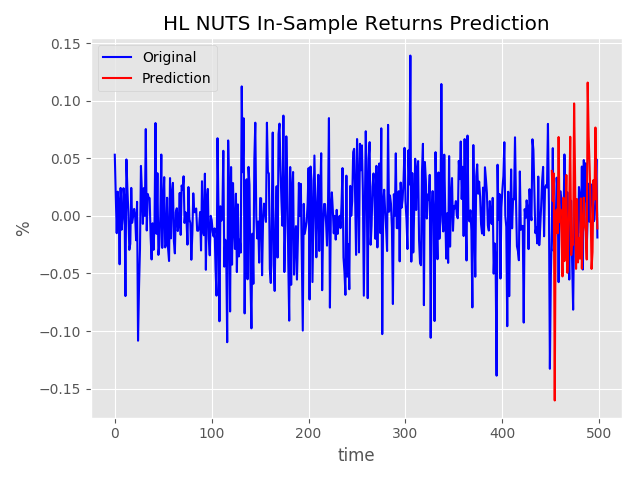
\includegraphics[width=\textwidth]{HL-NUTS-In-Sample-Returns-Prediction.png}
    \captionof{figure}{HL NUTS in-sample prediction}
    \label{fig:nonfloat}
\end{center}

\begin{center}  
    \includegraphics[width=\textwidth]{100-Day-HL-NUTS-Out-of-Sample-Returns-Forecast.png}
    \captionof{figure}{100 day HL NUTS out-of-sample forecast}
    \label{fig:nonfloat}
\end{center}

\section{Strategy}

\subsection{Classification}

\begin{center}
    \begin{tabular}{ | l | l | l | | l | l | l | p{5cm} |}
    \hline
    
    Starting Capital & \$100,000 \\ \hline
    Total Capital Used & \$103,110.65 \\ \hline
    Sharpe Ratio & 0.346 \\ \hline
    Portfolio Value & \$149,126.306 \\ \hline
    Algorithm Period Return & 0.491 \\ \hline
    Benchmark Period Return & 1.008 \\ \hline
    Algorithm Volatility & 0.272 \\ \hline
    Benchmark Volatility & 0.156 \\
    \hline
    \end{tabular}
    \captionof{table}{Machine Learning Classifier strategy with only upwards forecasts}
    \label{table:nonfloat}
\end{center}

\begin{center}  
    \includegraphics[width=\textwidth]{MLC-Portfolio-Benchmark-Up.png}
    \captionof{figure}{Machine Learning Classifier strategy with only upwards forecasts}
    \label{fig:nonfloat}
\end{center}

\begin{center}
    \begin{tabular}{ | l | l | l | | l | l | l | p{5cm} |}
    \hline
    Starting Capital & \$100,000 \\ \hline
    Total Capital Used & \$76,853.53 \\ \hline
    Sharpe Ratio & -0.548 \\ \hline
    Portfolio Value & \$20,134.519 \\ \hline
    Algorithm Period Return & -0.799 \\ \hline
    Benchmark Period Return & 1.008 \\ \hline
    Algorithm Volatility & 0.323 \\ \hline
    Benchmark Volatility & 0.156 \\
    \hline
    \end{tabular}
    \captionof{table}{Machine Learning Classifier strategy with upwarda and downwards forecasts}
    \label{table:nonfloat}
\end{center}

\begin{center}  
    \includegraphics[width=\textwidth]{MLC-Portfolio-Benchmark-Up-and-Down.png}
    \captionof{figure}{Machine Learning Classifier strategy with upwards and downwards forecasts}
    \label{fig:nonfloat}
\end{center}

\begin{center}
    \begin{tabular}{ | l | l | l | | l | l | l | p{5cm} |}
    \hline
    Starting Capital & \$100,000 \\ \hline
    Total Capital Used & \$295,844.66 \\ \hline
    Sharpe Ratio & 0.385 \\ \hline
    Portfolio Value & \$167,474.009 \\ \hline
    Algorithm Period Return & 0.675 \\ \hline
    Benchmark Period Return & 1.008 \\ \hline
    Algorithm Volatility & 0.393 \\ \hline
    Benchmark Volatility & 0.156 \\
    \hline
    \end{tabular}
    \captionof{table}{Machine Learning Classifier strategy with stop loss}
    \label{table:nonfloat}
\end{center}

\begin{center}  
    \includegraphics[width=\textwidth]{MLC-Portfolio-Benchmark-Stop-Loss.png}
    \captionof{figure}{Machine Learning Classifier strategy with stop loss}
    \label{fig:nonfloat}
\end{center}

\subsection{Regression}

\begin{center}
    \begin{tabular}{ | l | l | l | | l | l | l | p{5cm} |}
    \hline
    Starting Capital & \$100,000 \\ \hline
    Total Capital Used & \$229,547.84 \\ \hline
    Sharpe Ratio & 0.420 \\ \hline
    Portfolio Value & \$183,714.616 \\ \hline
    Algorithm Period Return & 0.837 \\ \hline
    Benchmark Period Return & 1.008 \\ \hline
    Algorithm Volatility & 0.373 \\ \hline
    Benchmark Volatility & 0.156 \\
    \hline
    \end{tabular}
    \captionof{table}{Machine Learning Regression strategy with only upwards forecasts}
    \label{table:nonfloat}
\end{center}

\begin{center}  
    \includegraphics[width=\textwidth]{MLR-Portfolio-Benchmark-Up.png}
    \captionof{figure}{Machine Learning Regression strategy with only upwards forecasts}
    \label{fig:nonfloat}
\end{center}

\begin{center}
    \begin{tabular}{ | l | l | l | | l | l | l | p{5cm} |}
    \hline
    Starting Capital & \$100,000 \\ \hline
    Total Capital Used & \$80,121.51 \\ \hline
    Sharpe Ratio & -0.258 \\ \hline
    Portfolio Value & \$19,628.34 \\ \hline
    Algorithm Period Return & -0.804 \\ \hline
    Benchmark Period Return & 1.008 \\ \hline
    Algorithm Volatility & 0.493 \\ \hline
    Benchmark Volatility & 0.156 \\
    \hline
    \end{tabular}
    \captionof{table}{Machine Learning Regression strategy with upwards and downwards forecasts}
    \label{table:nonfloat}
\end{center}

\begin{center}  
    \includegraphics[width=\textwidth]{MLR-Portfolio-Benchmark-Up-and-Down.png}
    \captionof{figure}{Machine Learning Regression strategy with upwards and downwards forecasts}
    \label{fig:nonfloat}
\end{center}

\begin{center}
    \begin{tabular}{ | l | l | l | | l | l | l | p{5cm} |}
    \hline
    Starting Capital & \$100,000 \\ \hline
    Total Capital Used & \$229,547.84 \\ \hline
    Sharpe Ratio & 0.420 \\ \hline
    Portfolio Value & \$183,714.616 \\ \hline
    Algorithm Period Return & 0.837 \\ \hline
    Benchmark Period Return & 1.008 \\ \hline
    Algorithm Volatility & 0.373 \\ \hline
    Benchmark Volatility & 0.156 \\
    \hline
    \end{tabular}
    \captionof{table}{Machine Learning Regression strategy with stop loss}
    \label{table:nonfloat}
\end{center}

\begin{center}  
    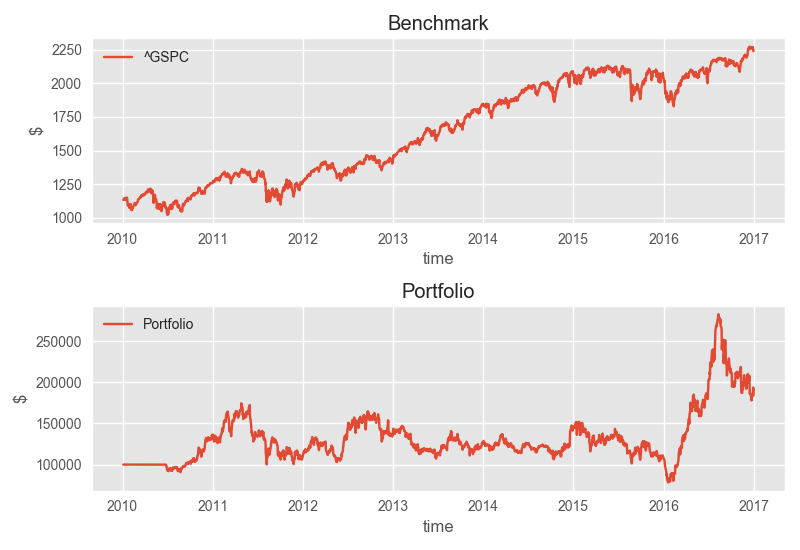
\includegraphics[width=\textwidth]{MLR-Portfolio-Benchmark-Stop-Loss.png}
    \captionof{figure}{Machine Learning Regression strategy with stop loss}
    \label{fig:nonfloat}
\end{center}